\documentclass[12pt, a4paper]{article}
\usepackage[english,russian]{babel}
\usepackage{csquotes}
\usepackage{graphicx}

\oddsidemargin=-0.4mm
\textwidth=160mm
\topmargin=4.6mm
\textheight=210mm
\parindent=0pt
\parskip=3pt

\begin{document}

    \begin{titlepage}

        \begin{center}

            \bfseries
            {\Large Московский авиационный институт\\ 
            (национальный исследовательский университет)}

            \vspace{48pt}
            {\large Факультет информационных технологий и прикладной 
            математики}
            
            \vspace{36pt}
            {\large Кафедра вычислительной математики и программирования}
            
            \vspace{48pt}
            Лабораторная работа \textnumero 1 по курсу 
            \enquote{Компьютерная графика}
            
        \end{center}
        
        \vspace{72pt}
        \begin{flushright}
            \begin{tabular}{rl}
                Студент: & В.\,Д. Молчанов   \\
                Преподаватель: & Л.\,Н. Чернышов \\
                Группа: & М8О-308Б-20 \\
                Дата: & \\
                Оценка: & \\
                Подпись: & \\
            \end{tabular}
        \end{flushright}
        
        \vfill
        
        \begin{center}
            
            \bfseries
            Москва, \the\year
        
        \end{center}

    \end{titlepage}
        
    \pagebreak

    \section*{Лабораторная работа \textnumero 1}

    \par\textbf{Тема: } {
        Построение изображений 2D-кривых.
    }

    \par\textbf{Задача: } {
        Написать и отладить программу, строящую изображение заданной 
        замечательной кривой.
    }

    \par\textbf{Вариант \textnumero 14: }
    $\rho= a * (1 - \cos(\phi))$
    
    \section{Решение}
    Для выполнения поставленной задачи было принято решение использовать язык 
    программирования Python и его модули matplotlib (для отрисовки графика и 
    координатных осей) и numpy. Из библиотеки numpy пригодилось $np.arange()$.
    Это функция создания массива с равномерно распределенным значениями на промежутках.
    Пользователю необходимо ввести число $a$. Полученный результат выводится на экран с 
    помощью функции show. Результат работы программы можно увидеть ниже.
    
    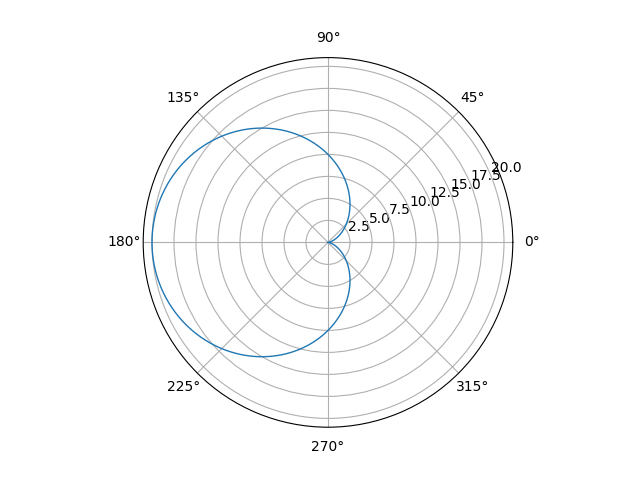
\includegraphics[scale=0.75]{Figure_1.png}
    
    \pagebreak
    
    \section{Выводы}
    Проделав лабораторную работу, познакомился с отрисовкой 2D-изображений, 
    нарисовал график в полярной системе координат, а также укрепил навыки 
    работы с matplotlib и numpy.

\end{document}